%! Tex program = xelatex
\documentclass{article}
%中文
\usepackage[UTF8]{ctex}
\usepackage[english]{babel}
%数学公式
\usepackage{amsmath,amssymb}
%\usepackage{ntheorem}
\usepackage{mdframed} %公式框1
% e.g., \newmdtheoremenv{theorem}{Theorem}
\usepackage{amsthm}
%边界
\usepackage[letterpaper,top=1cm,bottom=2cm,left=2cm,right=2cm,marginparwidth=1.75cm]{geometry}%table package
%Table
\usepackage{multirow,booktabs}
\usepackage{makecell}
%字体颜色
\usepackage{color}
\usepackage[dvipsnames]{xcolor}  % 更全的色系
%代码
\usepackage[OT1]{fontenc}
% MATLAB 代码风格
\usepackage[framed,numbered,autolinebreaks,useliterate]{/Users/anye_zhenhaoyu/Desktop/Latex/mcode}
\usepackage{listings}
\usepackage{algorithm}
\usepackage{algorithmic}
\usepackage{pythonhighlight} % Python
%插图
\usepackage{graphicx}
%改变item格式
\usepackage{enumerate}
%物理
\usepackage{physics}
%extra arrows
\usepackage{extarrows}
% caption(居中指令)
%\usepackage[justification=centering]{caption}
\usepackage{caption}
% htpb
\usepackage{stfloats}
% pdf 拼接
\usepackage{pdfpages}
% 超链接url
\usepackage{url}

\def\RR{\mathbb{R}}
\def\ZZ{\mathbb{Z}}
\def\EE{\mathbb{E}}

\def\Trsp#1{#1^{\mathcal{T}}}
\def\LT{\mathcal{L}}

\def\bold#1{\boldsymbol{#1}}
\def\bw{\boldsymbol{\omega}}
\def\ba{\boldsymbol{a}}
\def\bb{\boldsymbol{b}}
\def\bc{\boldsymbol{c}}
\def\bd{\boldsymbol{d}}
\def\be{\boldsymbol{e}}
\def\bf{\boldsymbol{f}}
\def\bg{\boldsymbol{g}}
\def\bh{\boldsymbol{h}}
\def\bt{\boldsymbol{t}}
\def\bu{\boldsymbol{u}}
\def\bv{\boldsymbol{v}}
\def\bx{\boldsymbol{x}}
\def\by{\boldsymbol{y}}
\def\bz{\boldsymbol{z}}

\def\bA{\boldsymbol{A}}
\def\bB{\boldsymbol{B}}
\def\bC{\boldsymbol{C}}
\def\bE{\boldsymbol{E}}
\def\bF{\boldsymbol{F}}
\def\bG{\boldsymbol{G}}
\def\bL{\boldsymbol{L}}
\def\bM{\boldsymbol{M}}
\def\bO{\boldsymbol{O}}
\def\bP{\boldsymbol{P}}
\def\bQ{\boldsymbol{Q}}
\def\bX{\boldsymbol{X}}
\def\bY{\boldsymbol{Y}}

\def\Esolve{\textcolor{blue}{Solve: }}
\def\Eproof{\textcolor{blue}{Proof: }}
\def\case#1{\textcolor{blue}{Case \uppercase\expandafter{\romannumeral#1}: }}

\def\suminf#1{\sum_{#1=-\infty}^{+\infty}}
\def\ft{\mathcal{F}}
\def\lt{\mathcal{L}}
\def\zt{\mathcal{Z}}


\newmdtheoremenv{prt}{{\color{PineGreen}Property}}
\newmdtheoremenv{thm}{\textcolor{red}{Theorem}}
\newmdtheoremenv{defi}{\textcolor{blue}{Definition}}

\graphicspath{{figures/}}

\begin{document}
\title{信号与系统简明笔记}
\author{Zhen Hy}
\maketitle
Available at \textcolor{blue}{\url{https://github.com/anyeZHY/Concise-Notes-SJTU-ICE2501}}.
\section*{\centering \color{Purple}总览(重要)}

\begin{thm}Transformations:
	\begin{enumerate}
		\item Fourier:
			\[
				\begin{cases}\displaystyle
					x(t)=\dfrac{1}{2\pi}\int_{-\infty}^{+\infty} X(\omega)e^{j\omega t}\dd\omega
					\\[10pt]\displaystyle
					X(\omega)=
					\int_{-\infty}^{+\infty} x(t)e^{-j\omega t}\dd t
				\end{cases}
			\]
		\item DTFT:
			\[
				\begin{cases}\displaystyle
					x(t)=\dfrac{1}{2\pi}
					\int_{2\pi}
					X(e^{j\omega})e^{j\omega n}\dd \omega
					\\[10pt]\displaystyle
					X(e^{j\omega})=
					\suminf{n}x[n]e^{-j\omega n}
				\end{cases}
			\]
		\item Laplace(逆变换不做要求,注意单边双边变换)
			\[
				X(s)=\int x(t)e^{-st}\dd t
			\]
		\item Z(逆变换不做要求,注意单边双边变换)
			\[
				X(z)=\sum_nx(n)z^{-n}
			\] 
	\end{enumerate}
\end{thm}


\begin{mdframed}
	{\color{Purple}一些有趣的方法:}
	\begin{itemize}
		\item 利用卷积求导、线性等性质把$x(t)$凑成$\delta(t)$,直接求$h(t)$
		\item 求导使两边复杂程度降低,减少变换难易程度。
		\item z平面零极点矢量作图法
		\item 有时直接解微分方程会更快......
	\end{itemize}
\end{mdframed}

\begin{table}[H]
	\centering
	\begin{tabular}{c|l|l|l|l}
		\Xhline{1pt}
		Properties & Input & Fourier & Laplace & Z
		\\[3pt]
		Original & $x(t)/x[n]$ & $X(\omega)$ & $X(s)$ & $X(z)$
		\\[2pt]\Xhline{1pt}
		线性 &  &  &  & 
		\\[7pt]
		时移 & $x(t-t_0)$ & $X(\omega)e^{-j\omega t_0}$ & $X(s)e^{-st_0}$ & $X(z)z^{-n_0}$
		\\[7pt]
		奇偶虚实 & $x^*(t)$ & $X^*(-\omega)$ & $X^*(s^*)$ & $X^*(z^*)$
		\\[7pt]
		积分 & $\displaystyle\int x(t)\dd t$ & 
		$\pi X(0)\delta(\omega)+\dfrac{X(\omega)}{j\omega}$ 
		& 
		$\displaystyle\frac{1}{s}\int_{-\infty}^{0^-}x(\tau)\dd\tau+\frac{1}{s}X(s)$ & $\dfrac{1}{1-z^{-1}}X(z)$
		\\[10pt]
		微分 & $x^{(n)}(t)$ & $(j\omega)^nX(\omega)$ & $sX(s)-x(0^{\bold{\color{Red}-}})$ & $(1-z^{-1})X(z)-x[-1]$
		\\[7pt]
		时间频率变换 & $x(at)$ & $\dfrac{1}{\abs{a}}X(\dfrac{\omega}{a})$ & $\dfrac{1}{\abs{a}}X(\dfrac{s}{a})$ & 
		\\[10pt]
		对偶性 & $X(t)$ & $2\pi x(-\omega)$ &  & 
		\\[7pt]
		频域微分 & $tx(t)$ & $j\dv*{X(\omega)}{\omega}$ & $-\dv*{X(s)}{s}$ & $z^{-1}\dv*{X(z)}{z^{-1}}$
		\\[7pt]
		频移 & $(e^{j\omega_0t}/e^{s_0t})x(t)$ & $X(\omega-\omega_0)$ & $X(s-s_0)$ & 
		\\[7pt]
		卷积 & $x_1*x_2$ & $X_1X_2$ & $X_1X_2$ & $X_1X_2$
		\\[7pt]
		乘积 & $x_1x_2$ & $\dfrac{1}{2\pi}X_1*X_2$ &  & 
		 \\[7pt]\Xhline{1pt}
	\end{tabular}
	\caption{不同变换的性质}
\end{table}

\begin{table}[H]
	\centering
	\begin{tabular}{c|ll}
		判断 & 因果性 & 稳定性 \\ \hline
		冲激响应$h(t)$ & $h(t)$为因果信号 & $\abs{\int h(t)\dd t}<+\infty$
		\\
		Laplace & $H(s)$有理函数,ROC在最右边极点的右边& 极点位于s平面的左半边(包含$j\omega$轴)。
		\\
		Z & ROC包括$\abs{z}=\infty$ & ROC包括单位圆
	\end{tabular}
	\caption{系统性质的判断}
\end{table}



\begin{defi}杂·知识点:
	\begin{enumerate}
		\item 模拟角频率$\Omega_0$;数字角频率$\omega_0\in[0,2\pi)$,$\pi$为最高频率
		\item $\Delta x[n]=x[n+1]-x[n]$, $\nabla x[n]=x[n]-x[n-1]$
		\item 卷积优先级高于乘法运算。
	\end{enumerate}
\end{defi}







\newpage
\section{信号函数表示、系统分析方法}
\begin{defi}
	信号基础定义:
	\begin{itemize}
		\item 连续/离散时间信号能量、功率
		\item 能量信号($E_{\infty}<\infty,\ P_\infty=0$)、功率信号($E_\infty=\infty,\ 0<P_\infty<\infty$)
		\item 模拟信号,脉冲信号(连续)。抽样信号、数字信号(离散)。
	\end{itemize}
\end{defi}
\begin{prt}
	一些特殊的信号:
	\begin{enumerate}
		\item 抽样信号$Sa(t)=\dfrac{\sin(t)}{t}$。$\int_0^{+\infty}Sa(\omega_0t)\dd t=\dfrac{\pi}{2}\dfrac{1}{\omega_0}$

		\item 阶跃函数$u(t)$、单位冲激函数$\delta(t)$,冲击偶函数(相关性质可用分部积分证明)。
			\begin{itemize}
				\item $\delta(t)=\dv*{[u(t)]}{t}$
				\item $\delta(at)=\flatfrac{\delta(t)}{\abs{a}}$,$\delta(f(t))=\sum_{f(t_i)=0}\dfrac{\delta(t_i)}{\abs{f'(t_i)}}$
				\item $x(t)*\delta(t-t_0)=x(t-t_0)$
			\end{itemize}
		\item $u[n]$从$n=0$开始。
	\end{enumerate}
\end{prt}

\begin{prt}系统的基本性质
	\begin{enumerate}
		\item 因果性:一个系统在任何时刻的输出都只与当时这个时刻的输入以及该时刻以前的输入有关
		\item 稳定性:输入有界、输出有界
		\item 时不变性:$\forall x:\mbox{s.t. }x(t)\to y(t),\mbox{ then } x(t-t_0)\to y(t-t_0)$
		\item 线性:可加性、其次性
		\item 增量线性系统、零输入响应、零状态响应
	\end{enumerate}
\end{prt}









\section{线性时不变系统的时域分析}

\begin{defi}
	单位样值响应$h[n]$、卷积
	$\sum_{k=-\infty}^{+\infty}x[k]h[n-k]$ or 
	$\int_{-\infty}^{+\infty}x(\tau)\delta(t-\tau)\dd\tau$
	(可以用Z变换法)
\end{defi}

\begin{prt}[卷积]
    交换率、分配律、结合律\\
	微分/积分性质:
	$\qty(\int x\dd\tau)*h=x*\qty(\int h\dd\tau)=\int y\dd\tau$\\
	时移性质:$x(t-t_0)*h(t)=x(t)*h(t-t_0)=y(t-t_0)$
\end{prt}

\begin{thm}[微分方程、差分方程]
    特解+通解(特征根)+初始条件
	\begin{table}[H]
		\centering
		\begin{tabular}{c|c|c}
			自由项 & 特征根情况 & 特解形式 \\ \hline
			$\delta[n]$ & & 0 \\
			常数 & 1不是特征根 & $A$\\
			常数 & 1是$k$重根 & $An^k$\\
			$n$的$p$次多项式 & 1不是特征根 & $n$的$p$次多项式\\
			$n$的$p$次多项式 & 1是$k$重根 & $n^k\times$($n$的$p$次多项式)
		\end{tabular}
	\end{table}
	通常不用处理$n,t<0$时的情况(除非题目要求)。
\end{thm}


\section{周期信号傅里叶级数表示}

\begin{thm}
	三角函数:\[x(t)=a_0+\sum_{n=1}^{+\infty}\qty[a_n\cos(n\omega_0t)+b_n\sin(n\omega_0t)]\]
	where
	\[
		a_n=\frac{2}{T_0}\int_0^{T_0}x(t)\cos(n\omega_0t)\dd t
	\] and 
	\[
		b_n=\frac{2}{T_0}\int_0^{T_0}x(t)\sin(n\omega_0t)\dd t
	.\] 
\end{thm}

\begin{thm}
	指数:
	\[
		x(t)=
		\sum_{n=-\infty}^{+\infty}
		\qty[X(n\omega)e^{jn\omega t}]
	\]
	where
	\[
		X(n\omega)=\frac{1}{T_0}\int_0^{T_0}x(t)e^{-jn\omega t}\dd t
	.\] 
\end{thm}

\begin{defi}
	$\abs{X(n\omega)}\sim\omega$偶函数,$\phi\sim\omega$奇函数(坑:$\pm\pi$)。直流分量、基波分量、高频分量。
\end{defi}

\begin{thm}[帕斯瓦尔定理]
    \[
		\frac{1}{T}\int_T\abs{x(t)}^2\dd t
		=
		\sum_{n=-\infty}^{+\infty}\abs{X(n\omega)}^2
    \] 
\end{thm}

\begin{defi}[频带宽度]
    一般把第一个零点定为频带宽度。
\end{defi}








\newpage
\section{连续时间信号的傅立叶变化}
Fourier Transformation定义、性质见总览。

\begin{thm}
	$x(t)$为实值偶函数,$X(\omega)$为实值偶函数。$x(t)$为实值奇函数,$X(\omega)$为虚奇函数。
    
\end{thm}

\begin{thm}
    \[
		\ft[x(t)]=\frac{1}{j\omega}\ft\qty[\dv{x(t)}{t}]+\pi\qty[x(-\infty)+x(+\infty)]\delta(\omega)
    \] 
\end{thm}

\begin{thm}[帕斯瓦尔定理]
    \[
		\int_{-\infty}^{+\infty}\abs{x(t)}^2\dd t=
		\frac{1}{2\pi}\int_{-\infty}^{+\infty}
		\abs{X(j\omega)}^2\dd\omega
    \] 
\end{thm}

\begin{defi}[采样]
	\[
		\delta_T(t)=\suminf{n}\delta(t-nT_s)\Longrightarrow
		\omega_s\suminf{n}\delta(\omega-n\omega_s)
	\]
	从而
	\[
		\ft[x(t)\delta_T(t)]=
		\frac{1}{T_s}\suminf{n}X(\omega-n\omega_s)
	\] 
	易知:
	$\omega_s\ge 2\omega_m$,$T_s\le\dfrac{1}{2f_m}$
\end{defi}




\section{连续时间系统的频域分析}

\begin{thm}Tricks:
	\begin{table}[H]
		\centering
		\begin{tabular}{c|ccccccccccc}
			输入 & $e^{j\omega_0t}$ & $\sin(\omega_0t)$
			\\[7pt]
			输出 & $H(j\omega_0)e^{j\omega_0t}$ & $\abs{H(j\omega_0)}\sin\qty[\omega_0t+\varphi(\omega_0)]$
		\end{tabular}
	\end{table}
\end{thm}


\begin{prt}线性不失真系统:
	\begin{enumerate}
		\item 幅频关系为一直线,通频带为无限宽。
		\item 相频关系是一个过原点负斜率直线。即群延时$\tau=-\dv*{\varphi(\omega)}{\omega}=Const$。(另注:相延时$t_f=\flatfrac{\varphi}{\omega}$,可参考物理中群速度和相速度定义。)
		\item 冲激响应是冲激函数。
	\end{enumerate}    
\end{prt}

\begin{defi}
    低通、高通、带通、带阻。通带、阻带。
	\\
	正弦幅度调制——移至频载位置(幅值减半)
\end{defi}






\section{DTFT}
引入:$\displaystyle x[n]=\sum_{k=0}^{N-1}a_ke^{jk\qty(\flatfrac{2\pi}{N})n}$。
易知:$X(e^{j\omega_0})$是以$2\pi$为周期的。
\begin{prt}[Z变换-DTFT]
	\textcolor{red}{{\textbf{$\star$Significant$\star$}}}:
	\[
		z^{-1}=e^{-j\omega}
	\]
	前提:Z变换ROC包括单位圆。
\end{prt}

\begin{prt}DTFT性质:
	\begin{itemize}
		\item 差分:$x[n]-x[n-1]\longleftrightarrow(1-e^{j\omega})X(e^{j\omega})$
		\item 求和:
			$
			\displaystyle\sum_{n=-\infty}^nx[k]=\frac{X}{1-e^{j\omega}}+\pi X(e^{j0})\suminf{k}\delta(\omega-2k\pi)
			$
	\end{itemize}
\end{prt}





\section{Laplace}
Laplace变换定义、性质见总览。
\begin{prt}ROC相关性质:
	\begin{itemize}
		\item ROC是S平面上平行于$j\omega$轴的带形区域。
		\item ROC内无极点
		\item 实现信号的ROC是整个平面
	\end{itemize}
\end{prt}

\begin{thm}初值定理与终值定理:
    \[
		\lim_{s\to+\infty}sX(s)=x(0^+)
		\mbox{ and }
		\lim_{s\to 0^+}sX(s)=x(+\infty)
	\]
\end{thm}
\newpage
\begin{thm}[部分分式展开法]这里以3为例:
    \[
		F(s)=\frac{A(s)}{B(s)(s+C)^3}=
		\frac{k_{11}}{(s+1)^3}+\frac{k_{12}}{(s+1)^2}
		+\frac{k_{13}}{s+1}+D(s)
    \] where
	\[
		\begin{aligned}
			k_{11}&=\eval{(s+1)^3F(s)}_{s=-1}
			\\[5pt]
			k_{12}&=\eval{\dv{s}\qty[(s+1)^3F(s)]}_{s=-1}
			\\[5pt]
			k_{13}&=\frac{1}{2}
			\eval{\dv[2]{s}\qty[(s+1)^3F(s)]}_{s=-1}
		\end{aligned}
	\] 
\end{thm}



\begin{prt}[DiracComb函数]
	$\delta_T(t)=\sum_{n=0}^{+\infty}\delta(t-nT)$. Thus 
	\[
		\lt[\delta_T(t)]=\frac{1}{1-e^{-Ts}}
	\] 
\end{prt}

\begin{defi}
    自由响应分量、强制响应分量。暂态响应、稳态响应。
\end{defi}

\begin{defi}[全通网络]幅频特性为常数;此时有极点位于左半平面,零点位于右半平面,极点零点关于$j\omega$轴对称。
\end{defi}

\begin{defi}[最小相移网络]
    此时零点位于左半平面或$j\omega$轴
\end{defi}

\begin{defi}[方框图]may be important:
	\[
		H(s)=\frac{2s^2+4s+6}{s^2+3s+2}
	\]
	\begin{figure}[H]
		\centering
		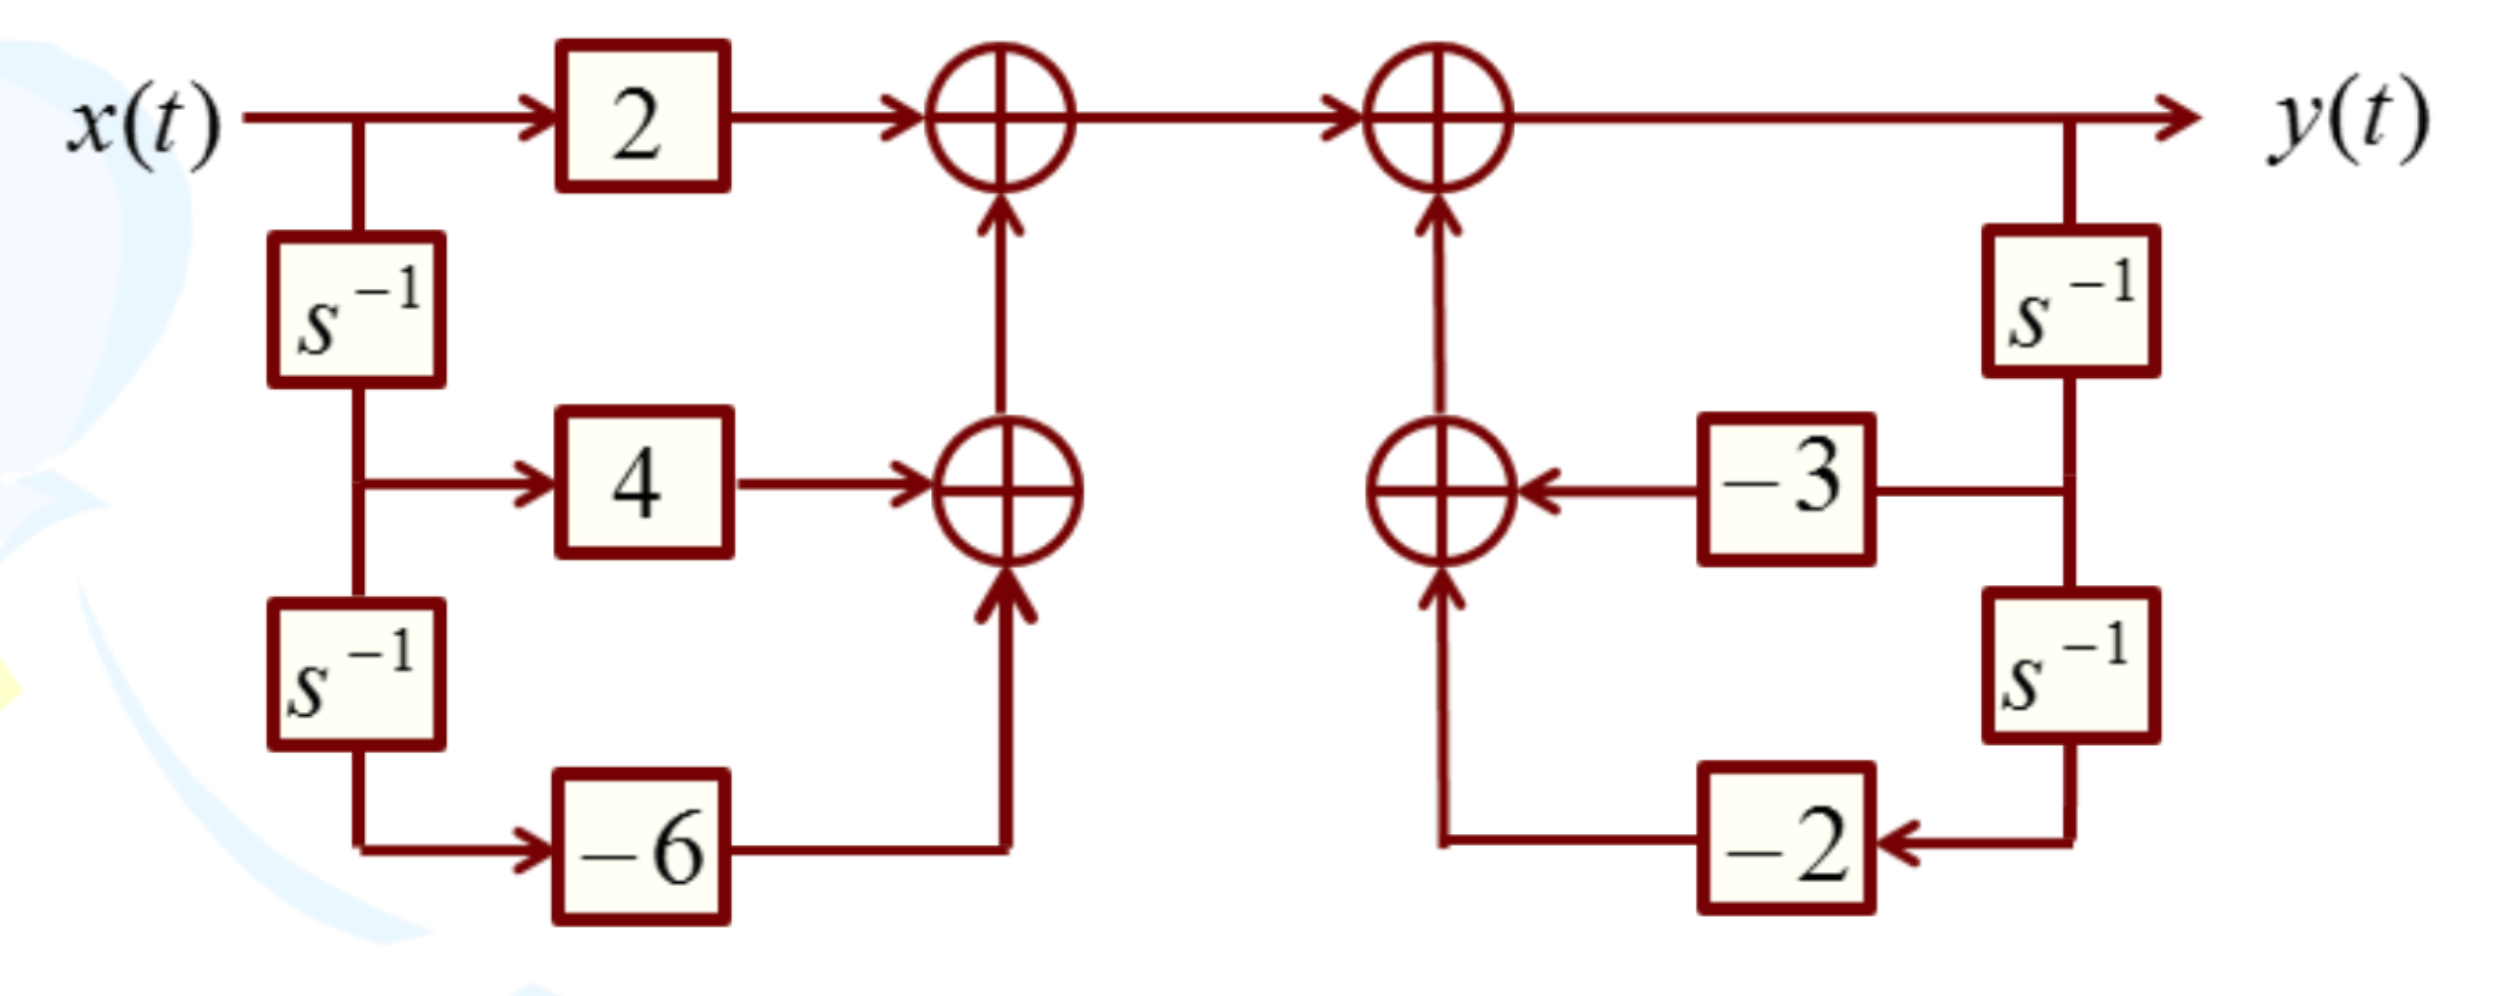
\includegraphics[width=0.7\linewidth]{直接.png}
		\caption{直接型}
	\end{figure}
	\begin{figure}[H]
		\centering
		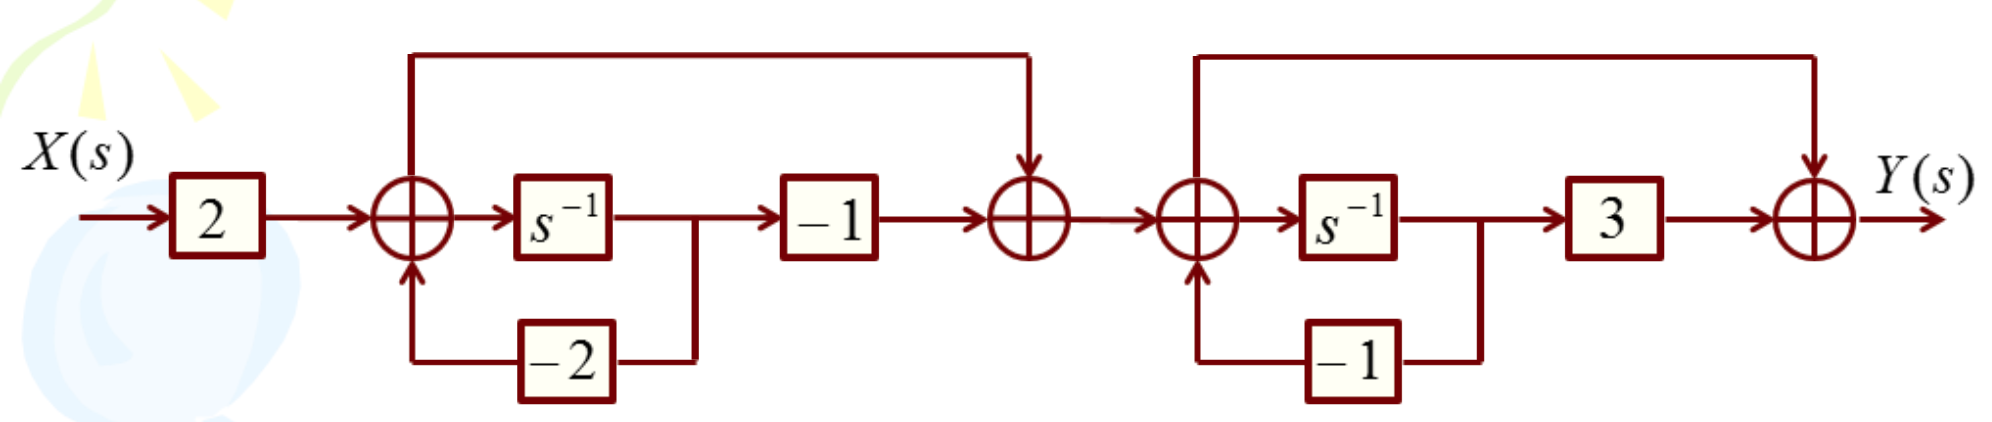
\includegraphics[width=0.7\linewidth]{级联.png}
		\caption{级联型}
	\end{figure}
	\begin{figure}[H]
		\centering
		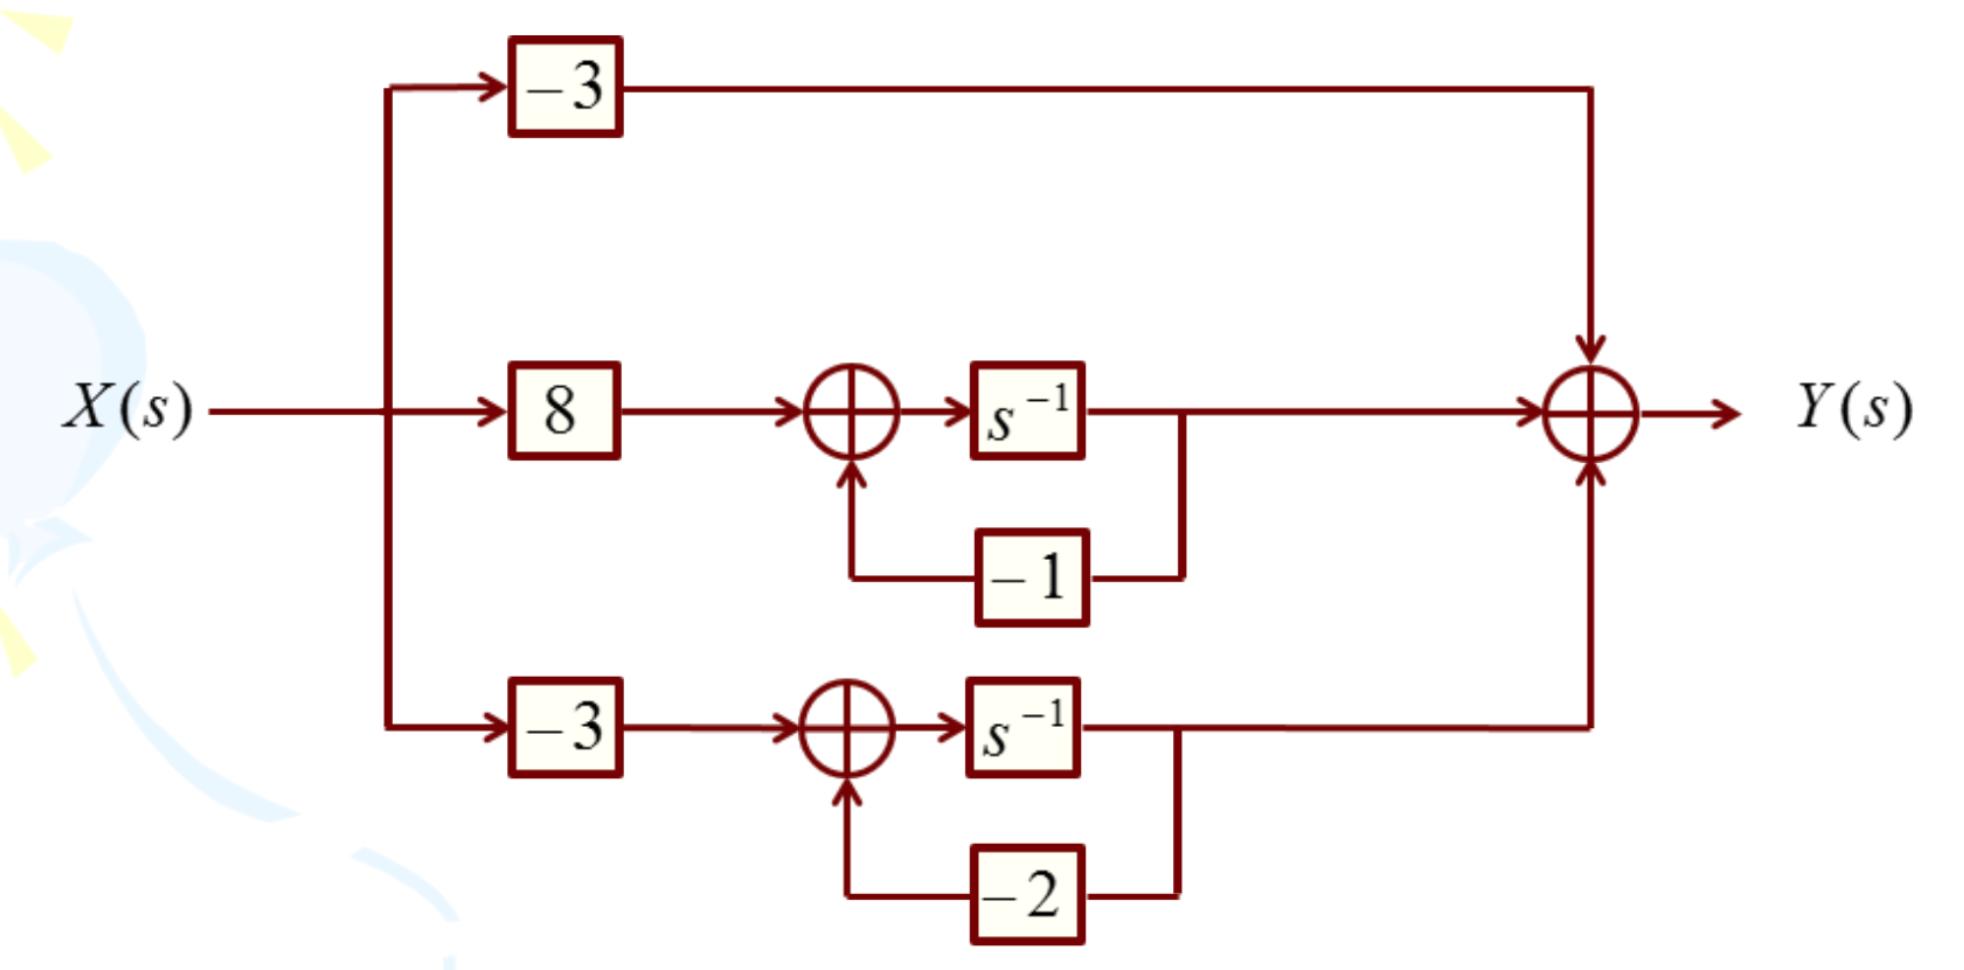
\includegraphics[width=0.7\linewidth]{并联.png}
		\caption{并联型}
	\end{figure}
\end{defi}

\section{Z}

\begin{defi}ROC:
	\begin{itemize}
		\item 圆环
		\item 有限长序列是整个z平面。
	\end{itemize}
\end{defi}

\begin{thm}[单边Z变换的位移性质]
	用于解释$x[n\pm1],x[n\pm2]$等。
	\\左位移:
	\[
		\zt\qty{x[n+m]u[n]}=
		z^{m}\qty{X(z)-\sum_{k=0}^{m-1}x[k]z^{-k}}
	\] 
	右位移:
    \[
		\zt\qty{x[n-m]u[n]}=
		z^{-m}\qty{X(z)+\sum_{k=-m}^{-1}x[k]z^{-k}}
    \]
	\textcolor{blue}{这是求解差分方程的基础}。e.g.,
	\[
	    \begin{aligned}
			\zt[x(n+2)]&=z^2X(z)-z^2x(0)-zx(1)
			\\
			\zt[x(n+1)]&=zX(z)-zx(0)
			\\
			\zt[x(n-1)]&=z^{-1}X(z)+x(-1)
			\\
			\zt[x(n-2)]&=z^{-2}X(z)+z^{-1}x(-1)+x(-2)
	    \end{aligned}
	\]
\end{thm}

\begin{thm}[Z域尺度变换]
    \[
		a^nx[n]\leftrightarrow X(\frac{z}{a})
    \] 
\end{thm}

\begin{prt}[重要性质]
	\textbf{\textcolor{red}{$\star$ Significant $\star$}}.
	\\
	If $x[n]\longleftrightarrow X(z)$, then
	\begin{itemize}
		\item 变换形式的一致性。$u[n]\Longrightarrow-u[-n-1]$
			\begin{table}[H]
				\centering
				\begin{tabular}{ccc}
					信号 & 变换 & 收敛域
					\\[6pt]
					$a^nu[n]$ & $\dfrac{1}{1-az^{-1}}$ & $\abs{z}>\abs{a}$
					\\[10pt]
					$-a^nu[-n-1]$ & $\dfrac{1}{1-az^{-1}}$ & $\abs{z}<\abs{a}$
				\end{tabular}
			\end{table}
		\item 时间反转(反演变换) 
			\[
				x[-n]\longleftrightarrow X(z^{-1})
			\]
		\item 初值定理
			\[
				x[0]=\lim_{z\to+\infty}X(z)
			\]
		\item 终值定理
			\[
				x[+\infty]=\lim_{z\to_1}(z-1)X(z)
			\] 
	\end{itemize}
\end{prt}

\begin{defi}[方框图]may be important:
	\[
		H(s)=\frac{2s^2+4s+6}{s^2+3s+2}
	\]
	\begin{figure}[H]
		\centering
		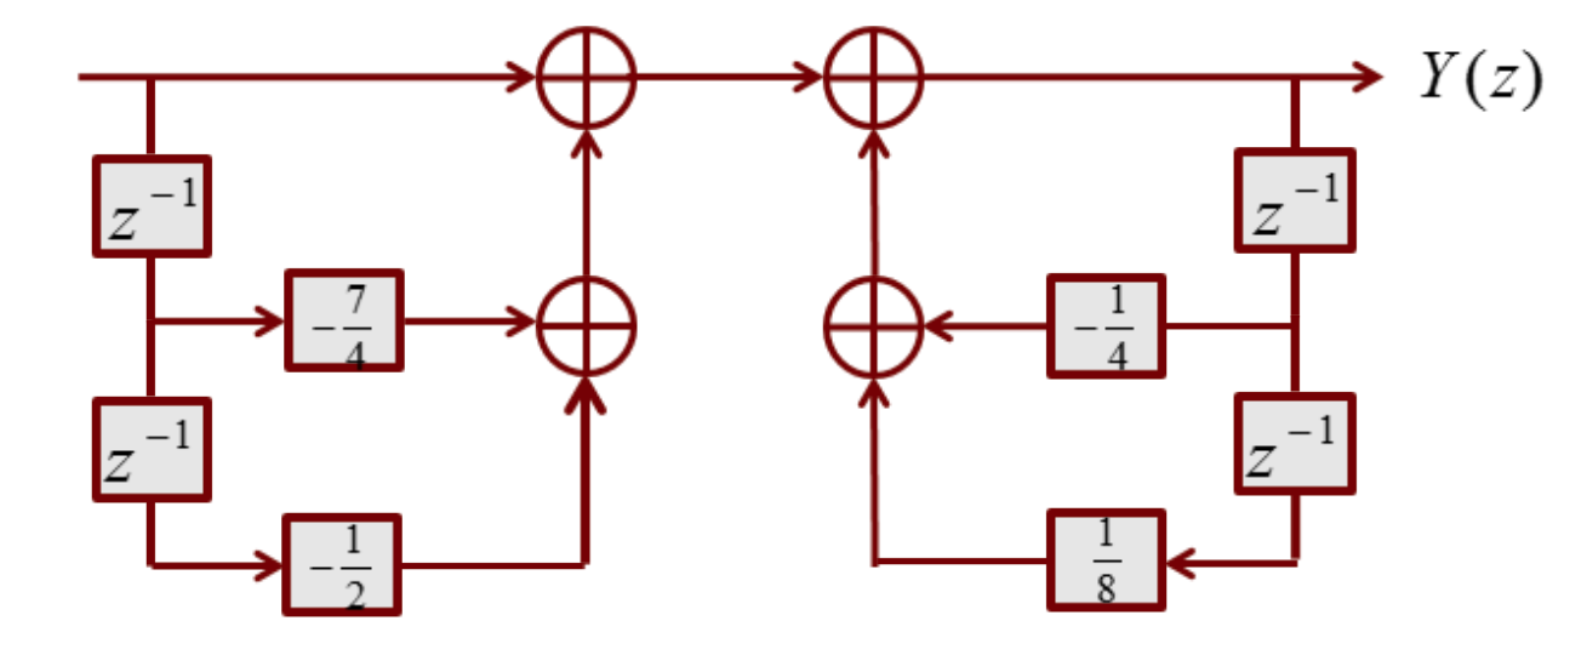
\includegraphics[width=0.7\linewidth]{z直接1.png}
		\caption{直接1型}
	\end{figure}
	\begin{figure}[H]
		\centering
		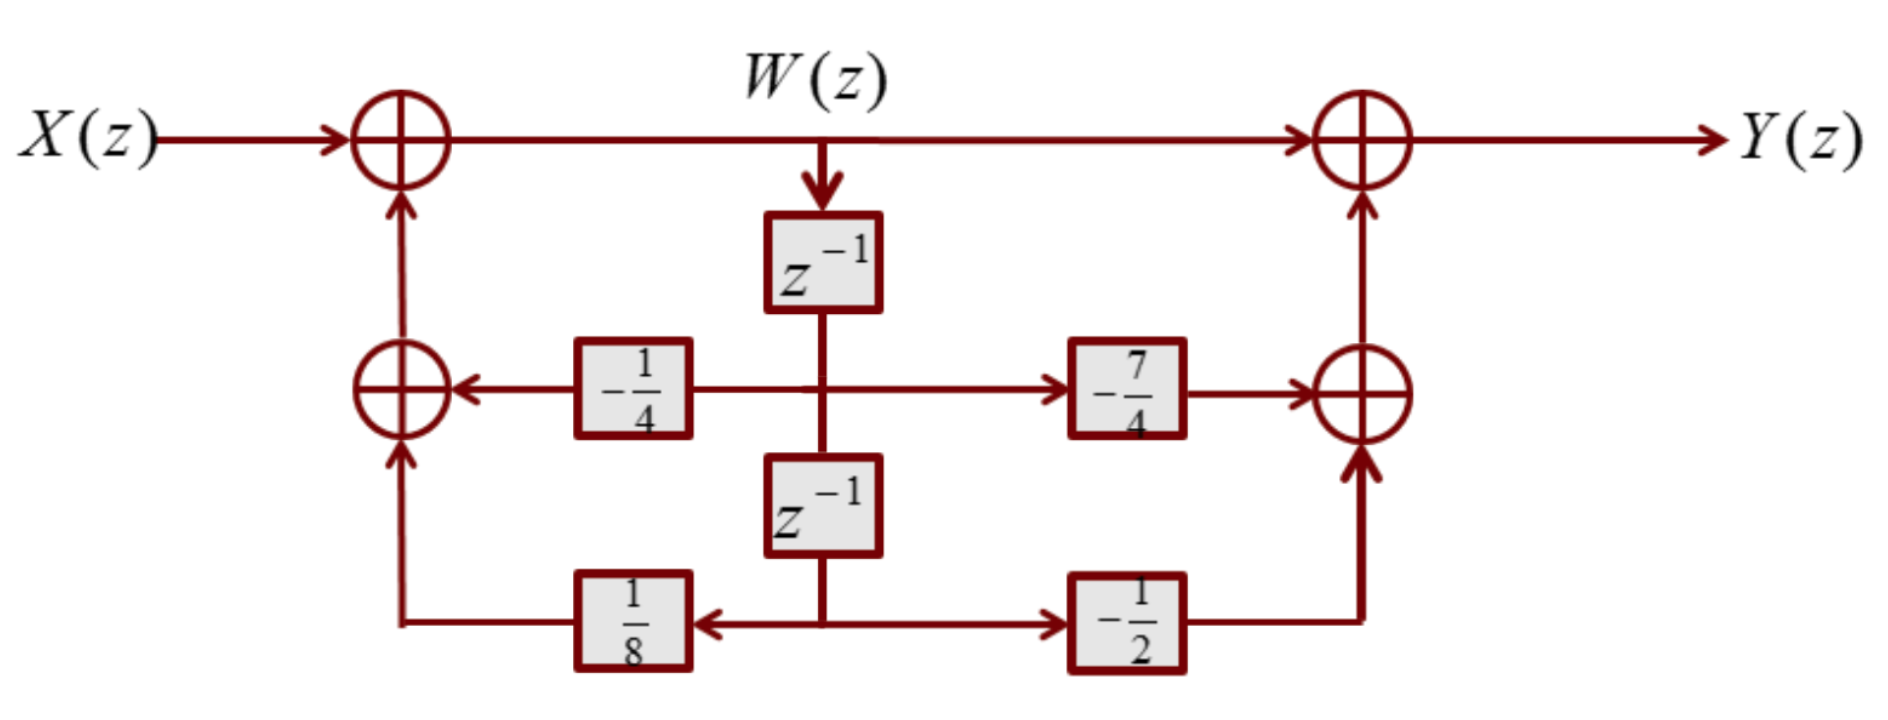
\includegraphics[width=0.7\linewidth]{z直接2.png}
		\caption{直接2型}
	\end{figure}
	\begin{figure}[H]
		\centering
		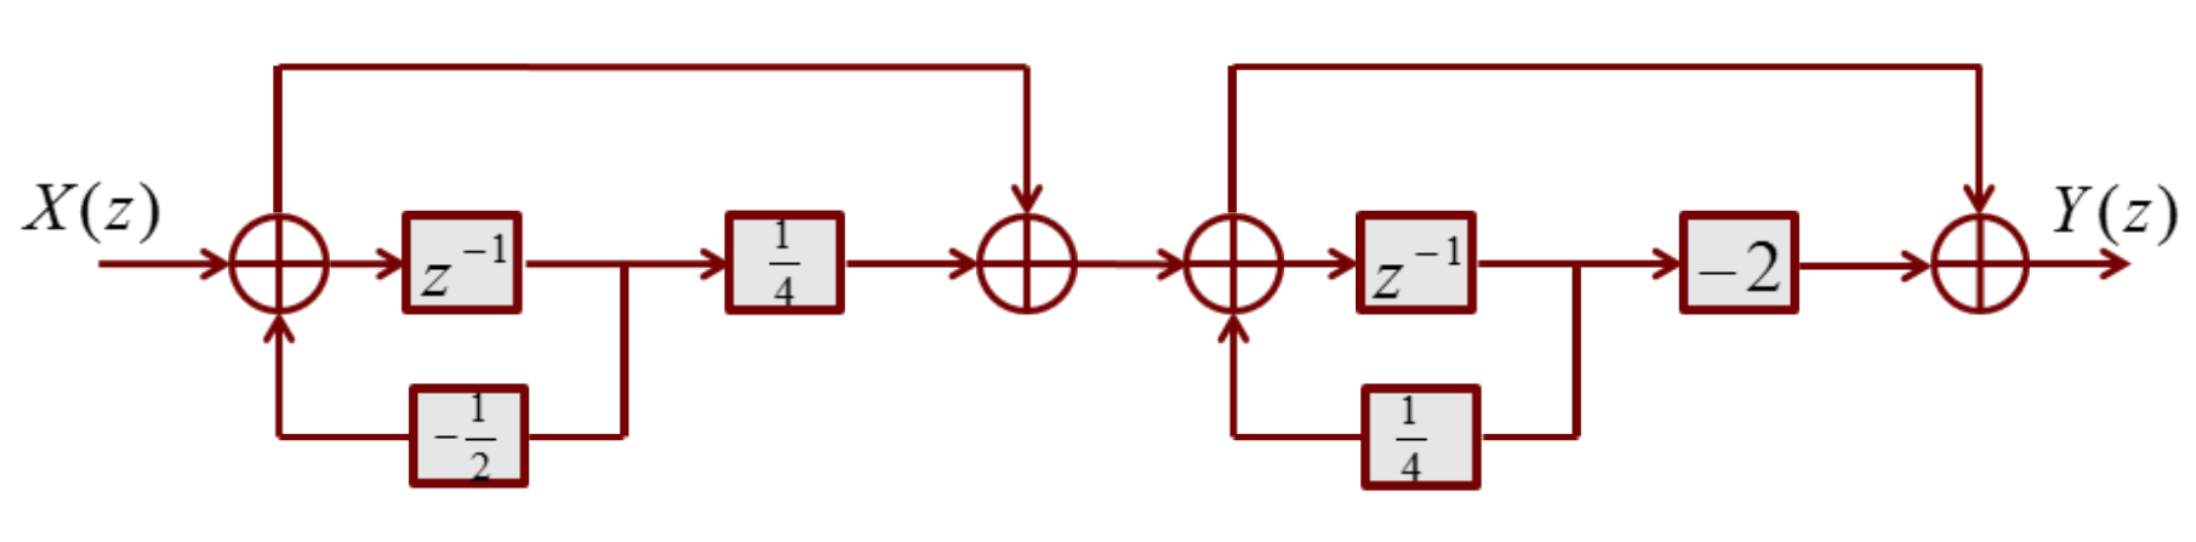
\includegraphics[width=0.7\linewidth]{z级联.png}
		\caption{级联型}
	\end{figure}
	\begin{figure}[H]
		\centering
		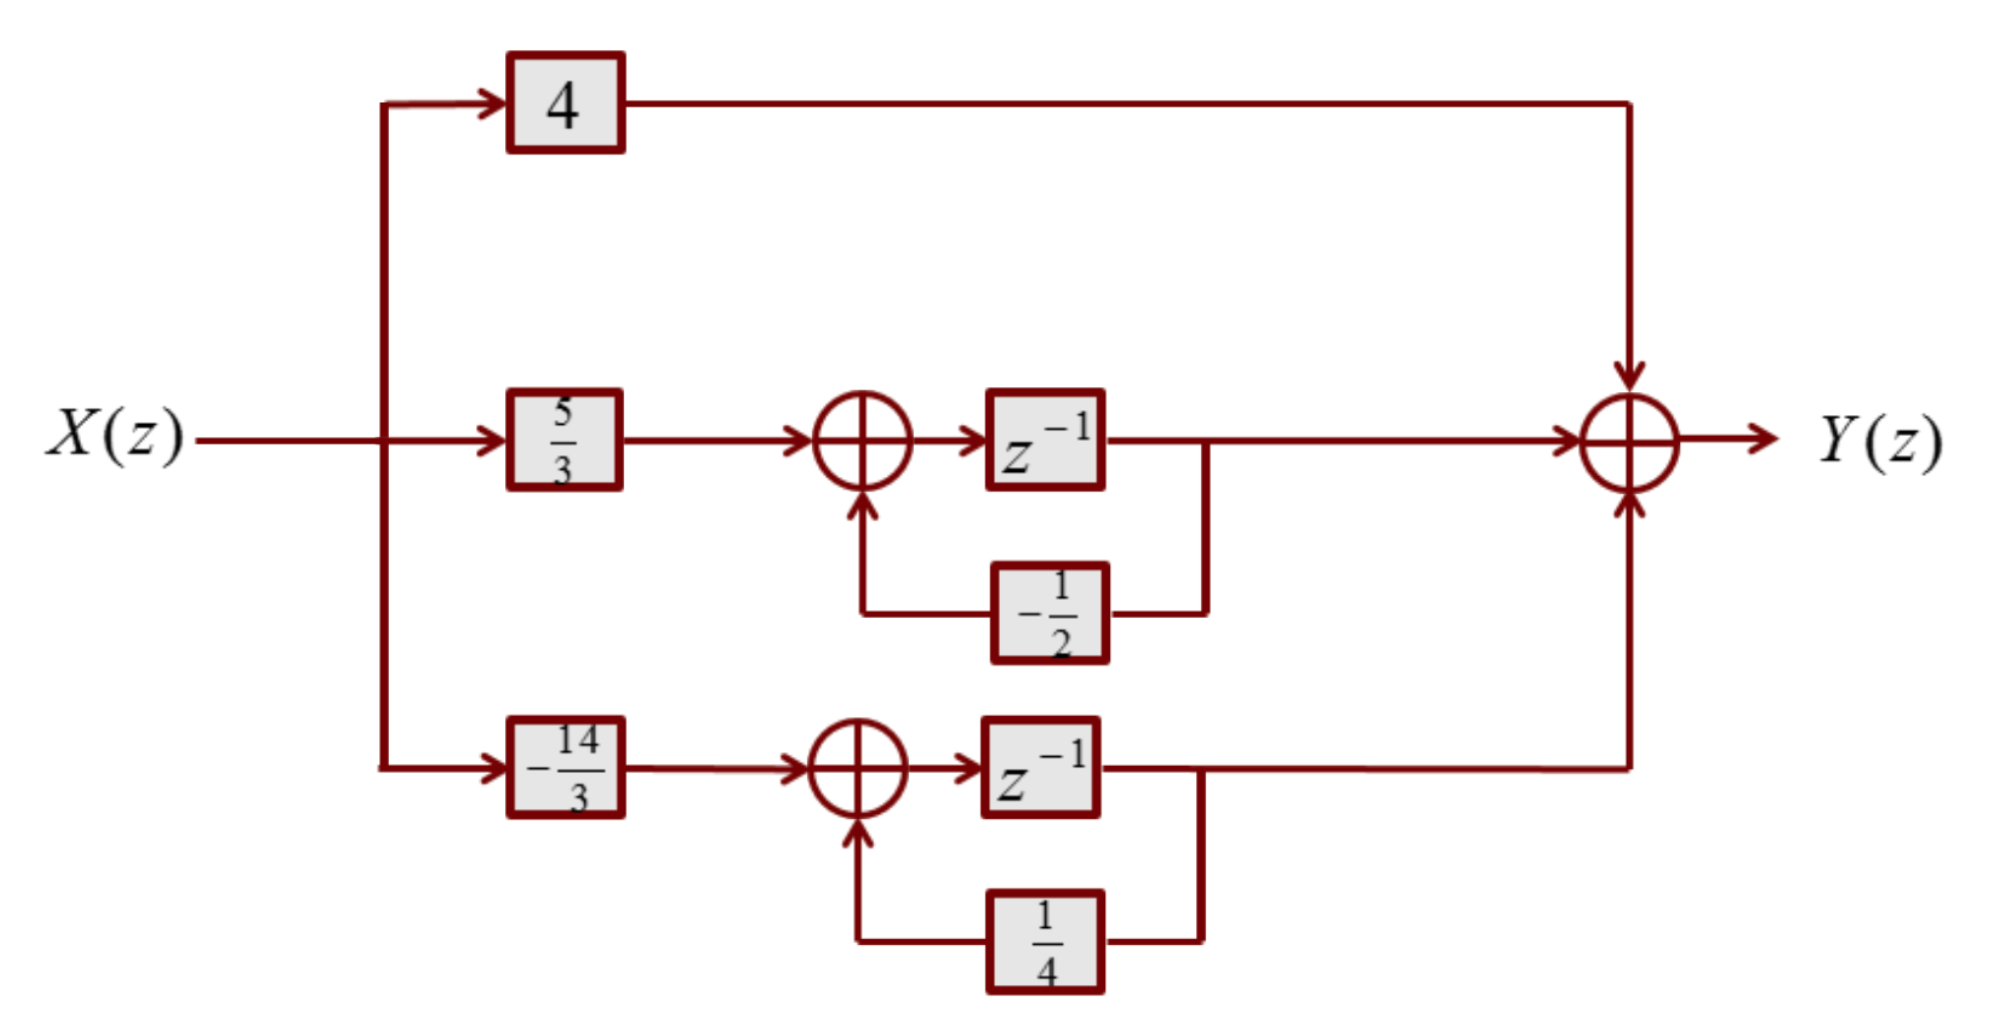
\includegraphics[width=0.7\linewidth]{z并联.png}
		\caption{并联型}
	\end{figure}
\end{defi}




\begin{thm}[拉普拉斯反变换]
    一些方法:
	\begin{enumerate}
		\item 部分分式法
		\item 幂级数展开(Taylor展开)
	\end{enumerate}
\end{thm}


\newpage
\section{其他}
\begin{thm}[陶冶情操]指大概率(100\%)不考:\\
	\begin{enumerate}
		\item 
			Dirichlet条件:
			信号绝对可积、有限个极值点、极值点有界、有限个间断点。\\
		\item
			Gibbs现象:
			用有限项傅里叶级数表示有间断点的信号时,在间断点附近不可避免的会出现振荡和超量。超量的幅度不会随所取项数的增加而减小。只是随着项数的增多,振荡频率变高,并向间断点处压缩,从而使它所占有的能量减少。
		\item 
			佩里维纳准则:
			物理可实现的充分必要条件:
			$\displaystyle
			\int_{-\infty}^{+\infty}
			\frac{\abs{\ln\abs{H(j\omega)}}}{1+\omega^2}
			\dd \omega
			$
	\end{enumerate}
    
	
\end{thm}


\end{document}

